\subsection{BÀI TẬP TRẮC NGHIỆM}
\Opensolutionfile{ans}[ans/1H4.B2]
\setcounter{ex}{0}

\begin{ex}%[Huỳnh Văn Quy]%[1H2Y2]
	Hai đường thẳng không có điểm chung thì
	\choice{chéo nhau}
	{song song}
	{cắt nhau}
	{\True chéo nhau hoặc song song}
\end{ex}

\begin{ex}%[Huỳnh Văn Quy]%[1H2Y2]
	Hai đường thẳng phân biệt không song song thì
	\choice{chéo nhau}
	{có điểm chung}
	{\True cắt nhau hoặc chéo nhau}
	{ không có điểm chung}
\end{ex}

\begin{ex}%[TLDH9-Lê Hồng Phi]%[1H2Y2-1]%
	Cho hai đường thẳng phân biệt không có điểm chung cùng nằm trong một mặt phẳng thì hai đường thẳng đó
	\choice
	{trùng nhau}
	{chéo nhau}
	{\True song song}
	{cắt nhau}
	\loigiai{
		Hai đường thẳng phân biệt không có điểm chung cùng nằm trong một mặt phẳng thì hai đường thẳng đó song song.}
\end{ex}

\begin{ex}%[Đề HKI Lớp 11, Lạc Long Quân, Khánh Hòa 2017-2018]%[Lê Hồng Phi - DA 11HK1-18]%[1H2Y2-1]%
	Chọn khẳng định {\bf sai}
	\choice
	{Hai đường thẳng phân biệt cùng song song với đường thẳng thứ ba thì song song với nhau}
	{Nếu hai đường thẳng chéo nhau thì chúng không đồng phẳng}
	{\True Hai đường thẳng song song thì không đồng phẳng và không có điểm chung}
	{Hai đường thẳng cắt nhau thì đồng phẳng và có một điểm chung}
	\loigiai{
		Khẳng định sai là \lq\lq  Hai đường thẳng song song thì không đồng phẳng và không có điểm chung\rq\rq.
	}
\end{ex}

\begin{ex}%[Ân Thọ]%[1H2B2]
	Cho đường thẳng $a$ cắt mặt phẳng $(P)$ tại điểm $A$. Mệnh đề nào sau đây đúng?
	\choice
	{Mọi đường thẳng nằm trong $(P)$ đều chéo với $a$}
	{Mọi đường thẳng nằm trong $(P)$ đều cắt $a$}
	{\True Mọi đường thẳng nằm trong $(P)$ hoặc chéo với $a$, hoặc cắt $a$}
	{Mọi đường thẳng nằm trong $(P)$ đều không cắt $a$}
\end{ex}

\begin{ex}%[Ân Thọ]%[1H2B2]
	% \immini[thm]{
		Cho tứ diện $ABCD$. Gọi $M$ và $N$ là hai điểm phân biệt nằm trên đường thẳng $AB$, $M'$ và $N'$ là hai điểm phân biệt nằm trên đường thẳng $CD$. Các mệnh đề sau đây, mệnh đề nào đúng?	
		\choice
		{Hai đường thẳng $MM'$ và $NN'$ có thể cắt nhau}
		{Hai đường thẳng $MM'$ và $NN'$ có thể song song với nhau}
		{Hai đường thẳng $MM'$ và $NN'$ hoặc cắt nhau hoặc song song với nhau}
		{\True Hai đường thẳng $MM'$ và $NN'$ chéo nhau}
	% }{\begin{tikzpicture}[line cap=round,line join=round,>=stealth,x=0.75cm,y=0.75cm]
	% 	\draw (0.0,-0.0)-- (2.0,-2.0);
	% 	\draw (2.0,-2.0)-- (5.0,0.0);
	% 	\draw (5.0,0.0)-- (3.0,3.0);
	% 	\draw (3.0,3.0)-- (0.0,-0.0);
	% 	\draw (3.0,3.0)-- (2.0,-2.0);
	% 	%\draw [dash pattern=on 2pt off 2pt] (1.5,1.5)-- (3.5,-1.0);
	% 	\draw [dash pattern=on 2pt off 2pt] (0.0,-0.0)-- (5.0,0.0);
	% 	\begin{scriptsize}
	% 	\draw [fill=black] (0.0,-0.0) circle (1pt);
	% 	\draw[color=black] (-0.06,0.2) node {$B$};
	% 	\draw [fill=black] (2.0,-2.0) circle (1pt);
	% 	\draw[color=black] (1.7,-1.95) node {$C$};
	% 	\draw [fill=black] (5.0,0.0) circle (1pt);
	% 	\draw[color=black] (5.07,0.15) node {$D$};
	% 	\draw [fill=black] (3.0,3.0) circle (1pt);
	% 	\draw[color=black] (3.2,3.0) node {$A$};
	% 	\end{scriptsize}
	% 	\end{tikzpicture}
	% }
\end{ex}

\begin{ex}%[Nguyễn Tiến Thùy]%[1H2B2]
	Cho tứ diện $ABCD$, lấy $M, N$ lần lượt là trung điểm của $CD, AB$. Khi đó, xác định vị trí tương đối giữa hai đường thẳng $BC$ và $MN$.
	\choice
	{\True Chéo nhau}
	{Có hai điểm chung}	
	{Song song}	
	{Cắt nhau}
\end{ex}

\begin{ex}%[Nguyễn Tiến Thùy]%[1H2B2]
	Cho tứ diện $MNPQ$. Mệnh đề nào trong các mệnh đề dưới đây là đúng?
	\choice
	{$MN\parallel PQ$}
	{$MN$ cắt $PQ$}
	{$MN$ và $PQ$ đồng phẳng}	
	{\True $MN$ và $PQ$ chéo nhau}
\end{ex}

\begin{ex}%[Nguyễn Tiến Thùy]%[1H2B2]
	Cho hình chóp $S.ABCD$, đáy $ABCD$ là hình bình hành. Điểm $M$ thuộc cạnh $SC$ sao cho $SM=3MC$, $N$ là giao điểm của $SD$ và $(MAB)$. Khi đó tứ giác $ABMN$ là hình gì?
	\choice
	{Tứ giác không có cặp cạnh nào song song}
	{Hình vuông}
	{\True Hình thang}
	{Hình bình hành}
\end{ex}

\begin{ex}%[Nguyễn Tiến Thùy]%[1H2B2]
	Cho hình chóp $S.ABCD$ có đáy $ABCD$ là hình thang $AB\parallel CD$. Gọi $d$ là giao tuyến của hai mặt phẳng $(ASB)$ và $(SCD)$. Khẳng định nào sau đây là đúng?
	\choice
	{\True $d\parallel AB$}
	{$d$ cắt $AB$}
	{$d$ cắt $AD$}	
	{$d$ cắt $CD$}
\end{ex}

\begin{ex}%[Huỳnh Văn Quy]%[1H2B2]
	Cho hình chóp $S.ABCD$. Gọi $G$, $E$ lần lượt là trọng tâm các tam giác $SAD$ và $SCD$. Lấy $M$, $N$ lần lượt là trung điểm $AB$, $BC$ . Khi đó ta có:
	\choice
	{$GE$ và $MN$ trùng nhau}	
	{$GE$ và $MN$ chéo nhau}
	{\True $GE$ và $MN$ song song với nhau}
	{$GE$ cắt $BC$}
	\loigiai{Gọi $I$ là trung điểm của $SD$. Xét tam giác $IAC$ có: $\dfrac{IG}{IA}=\dfrac{IE}{IC}=\dfrac{1}{3}$.
		\immini{Theo định lí đảo của định lí Thalet, ta có $GE||AC$\quad (1).\\
			Mặt khác, ta có $MN$ là đường trung bình của $\triangle ABC$ nên suy ra $MN||AC$\quad (2).\\
			Từ (1) và (2) ta có $MN||GE$}
		{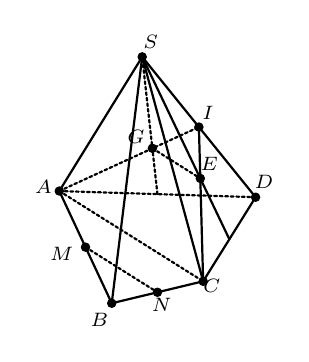
\begin{tikzpicture}[scale=1.5,line cap=round,line join=round,>=stealth,x=1.0cm,y=1.0cm]
			\draw [line width=0.8pt,dash pattern=on 1pt off 1pt] (0.539,2.203)-- (2.201,2.151);
			\draw [line width=0.8pt] (0.539,2.203)-- (0.983,1.253);
			\draw [line width=0.8pt] (0.983,1.253)-- (1.757,1.439);
			\draw [line width=0.8pt] (1.757,1.439)-- (2.201,2.151);
			\draw [line width=0.8pt] (1.241,3.339)-- (0.539,2.203);
			\draw [line width=0.8pt] (1.241,3.339)-- (2.201,2.151);
			\draw [line width=0.8pt] (1.241,3.339)-- (1.757,1.439);
			\draw [line width=0.8pt] (1.241,3.339)-- (0.983,1.253);
			\draw [line width=0.8pt,dash pattern=on 1pt off 1pt] (0.539,2.203)-- (1.757,1.439);
			\draw [line width=0.8pt,dash pattern=on 1pt off 1pt] (0.761,1.728)-- (1.370,1.346);
			\draw [line width=0.8pt] (1.721,2.745)-- (1.757,1.439);
			\draw [line width=0.8pt] (1.979,1.795)-- (1.241,3.339);
			\draw [line width=0.8pt,dash pattern=on 1pt off 1pt] (1.370,2.177)-- (1.241,3.339);
			\draw [line width=0.8pt,dash pattern=on 1pt off 1pt] (1.327,2.565)-- (1.733,2.310);
			\draw [line width=0.8pt,dash pattern=on 1pt off 1pt] (0.539,2.203)-- (1.721,2.745);
			\begin{scriptsize}
			\draw [fill=black] (0.539,2.203) circle (1.0pt);
			\draw[color=black] (0.404,2.239) node {$A$};
			\draw [fill=black] (2.201,2.151) circle (1.0pt);
			\draw[color=black] (2.273,2.281) node {$D$};
			\draw [fill=black] (0.983,1.253) circle (1.0pt);
			\draw[color=black] (0.879,1.114) node {$B$};
			\draw [fill=black] (1.757,1.439) circle (1.0pt);
			\draw[color=black] (1.829,1.403) node {$C$};
			\draw [fill=black] (1.241,3.339) circle (1.0pt);
			\draw[color=black] (1.313,3.468) node {$S$};
			\draw [fill=black] (1.721,2.745) circle (1.0pt);
			\draw[color=black] (1.798,2.869) node {$I$};
			\draw [fill=black] (1.370,1.346) circle (1.0pt);
			\draw[color=black] (1.406,1.238) node {$N$};
			\draw [fill=black] (0.761,1.728) circle (1.0pt);
			\draw[color=black] (0.559,1.671) node {$M$};
			\draw [fill=black] (1.733,2.310) circle (1.0pt);
			\draw[color=black] (1.809,2.435) node {$E$};
			\draw [fill=black] (1.327,2.565) circle (1.0pt);
			\draw[color=black] (1.189,2.663) node {$G$};
			\end{scriptsize}
			\end{tikzpicture}}}
\end{ex}

\begin{ex}%[Ân Thọ]%[1H2B2]
	\immini[thm]{Cho tứ diện $ABCD$ có $P, Q$ lần lượt là trọng tâm tam giác $ABC$ và $BCD$. Xác định giao tuyến của mặt phẳng $(ABQ)$ và mặt phẳng $(CDP)$.
		\choice
		{\True Giao tuyến là đường thẳng đi qua trung điểm hai cạnh $AB$ và $CD$}
		{Giao tuyến là đường thẳng đi qua trung điểm hai cạnh $AB$ và $AD$}
		{Giao tuyến là đường thẳng $PQ$}
		{Giao tuyến là đường thẳng $QA$}}
	{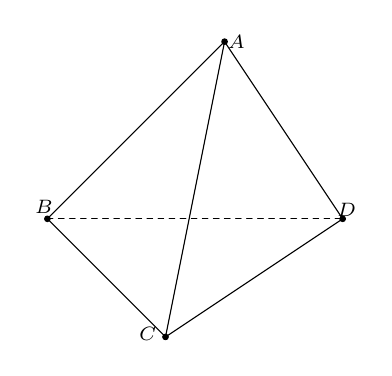
\begin{tikzpicture}[line cap=round,line join=round,>=stealth,x=0.75cm,y=0.75cm]
		\draw (0.0,-0.0)-- (2.0,-2.0);
		\draw (2.0,-2.0)-- (5.0,0.0);
		\draw (5.0,0.0)-- (3.0,3.0);
		\draw (3.0,3.0)-- (0.0,-0.0);
		\draw (3.0,3.0)-- (2.0,-2.0);
		%\draw [dash pattern=on 2pt off 2pt] (1.5,1.5)-- (3.5,-1.0);
		\draw [dash pattern=on 2pt off 2pt] (0.0,-0.0)-- (5.0,0.0);
		\begin{scriptsize}
		\draw [fill=black] (0.0,-0.0) circle (1pt);
		\draw[color=black] (-0.06,0.2) node {$B$};
		\draw [fill=black] (2.0,-2.0) circle (1pt);
		\draw[color=black] (1.7,-1.95) node {$C$};
		\draw [fill=black] (5.0,0.0) circle (1pt);
		\draw[color=black] (5.07,0.15) node {$D$};
		\draw [fill=black] (3.0,3.0) circle (1pt);
		\draw[color=black] (3.2,3.0) node {$A$};
		\end{scriptsize}
		\end{tikzpicture}
	}
\end{ex}

\begin{ex}%[1H2B2-2]
	Cho tứ diện $ABCD.$ Gọi $I$ và $J$ theo thứ tự là trung điểm của $AD$ và $AC,G$ là trọng tâm tam giác $BCD.$ Giao tuyến của hai mặt phẳng $\left(GIJ\right)$ và $\left(BCD\right)$ là đường thẳng
	\choice
	{qua $J$ và song song với $BD$}
	{qua $G$ và song song với $BC$}
	{qua $I$ và song song với $AB$}
	{\True qua $G$ và song song với $CD$}
	\loigiai{
		\immini{
			Ta có $\heva{
				& \left(GIJ\right)\cap \left(BCD\right)=G \\
				& IJ\subset \left(GIJ\right),\ CD\subset \left(BCD\right) \\
				& IJ\parallel CD}$\\
			$\Rightarrow \left(GIJ\right)\cap \left(BCD\right)=Gx\parallel IJ\parallel CD.$
		}
		{
			\begin{tikzpicture}[scale=0.7, line join=round, line cap=round]
			\tkzDefPoints{0/0/C,1.5/-1.8/B,4/0/D,2/3/A}
			\tkzDefMidPoint(A,C)\tkzGetPoint{J}
			\tkzDefMidPoint(D,A)\tkzGetPoint{I}
			\tkzCentroid(D,B,C)\tkzGetPoint{G}
			\tkzDefLine[parallel=through G](D,C)\tkzGetPoint{g}
			\tkzInterLL(g,G)(C,B)\tkzGetPoint{E}
			\tkzInterLL(g,G)(D,B)\tkzGetPoint{F}
			\tkzDrawPolygon(A,C,B,D)
			\tkzDrawSegments(A,B)
			\tkzDrawSegments[dashed](C,D I,J E,F)
			\tkzDrawPoints[fill=black](I,A,B,C,D,J,G)
			\tkzLabelPoints[above](A)
			\tkzLabelPoints[below](B,G)
			\tkzLabelPoints[left](C,J)
			\tkzLabelPoints[right](D,I)
			\end{tikzpicture}
		}
	}
\end{ex}

\begin{ex}%[1H2B2-2]
	Cho hình chóp $S.ABCD$ có đáy là hình thang với các cạnh đáy là $AB$ và $CD.$ Gọi $\left(ACI\right)$ lần lượt là trung điểm của $AD$ và $BC$ và $G$ là trọng tâm của tam giác $SAB.$ Giao tuyến của $\left(SAB\right)$ và $\left(IJG\right)$ là
	\choice
	{đường thẳng qua $S$ và song song với $AB$}
	{\True đường thẳng qua $G$ và song song với $DC$}
	{$SC$}
	{đường thẳng qua $G$ và cắt $BC$}
	\loigiai{
		\immini{
			Ta có: $I,J$ lần lượt là trung điểm của $AD$ và $BC$
			$\Rightarrow IJ$ là đường trung bình của hình thang $ABCD\Rightarrow IJ\parallel AB\parallel CD.$ \\
			Gọi $d=\left(SAB\right)\cap \left(IJG\right)$
			Ta có: $G$ là điểm chung giữa hai mặt phẳng $\left(SAB\right)$ và $\left(IJG\right)$ \\
			Mặt khác: $\heva{
				& \left(SAB\right)\supset AB;\left(IJG\right)\supset IJ \\
				& AB\parallel IJ \\}$ \\
			$\Rightarrow $Giao tuyến $d$ của $\left(SAB\right)$ và $\left(IJG\right)$ là đường thẳng qua $G$ và song song với $AB$ và $IJ.$
		}
		{
			\begin{tikzpicture}[scale=1, line join=round, line cap=round]
			\tkzDefPoints{0/0/A,0.5/-2/D,3.5/-2/C,5/0/B,2/3/S}
			\tkzDefMidPoint(B,C)\tkzGetPoint{J}
			\tkzDefMidPoint(D,A)\tkzGetPoint{I}
			\tkzCentroid(S,B,A)\tkzGetPoint{G}
			\tkzDefLine[parallel=through G](A,B)\tkzGetPoint{g}
			\tkzInterLL(g,G)(S,B)\tkzGetPoint{Q}
			\tkzInterLL(g,G)(S,A)\tkzGetPoint{P}
			\tkzDrawPolygon(S,A,D,C,B)
			\tkzDrawSegments(S,D S,C)
			\tkzDrawSegments[dashed](A,B I,J P,Q I,G J,G)
			\tkzDrawPoints[fill=black](I,A,B,C,D,J,G,S,P,Q)
			\tkzLabelPoints[above](S)
			\tkzLabelPoints[above left](G)
			\tkzLabelPoints[below](C,D)
			\tkzLabelPoints[left](A,I,P)
			\tkzLabelPoints[right](B,J,Q)
			\end{tikzpicture}
		}
	}
\end{ex}

\begin{ex}%[1H2B2-2]
	Cho hình chóp $S.ABCD$ có đáy $ABCD$ là hình bình hành. Gọi $I,J,E,F$ lần lượt là trung điểm $SA,SB,SC,SD.$ Trong các đường thẳng sau, đường thẳng nào không song song với $IJ?$
	\choice
	{$DC$}
	{$AB$}
	{\True $AD$}
	{$EF$}
	\loigiai{
		\immini{
			Ta có $IJ\parallel AB$ (tính chất đường trung bình trong tam giác $SAB$) và $EF\parallel CD$ (tính chất đường trung bình trong tam giác $SCD$).\\
			Mà $CD\parallel AB$ (đáy là hình bình hành)\\ $\Rightarrow CD\parallel AB\parallel EF\parallel IJ.$
		}
		{
			\begin{tikzpicture}[scale=0.7, line join=round, line cap=round]
			\tkzDefPoints{0/0/A,-1.5/-1.8/B,4/0/D, 0.2/3/S}
			\coordinate (C) at ($(B)+(D)-(A)$);
			\tkzDefMidPoint(A,S)\tkzGetPoint{I}
			\tkzDefMidPoint(B,S)\tkzGetPoint{J}
			\tkzDefMidPoint(C,S)\tkzGetPoint{E}
			\tkzDefMidPoint(D,S)\tkzGetPoint{F}
			\tkzDrawPolygon(S,B,C,D)
			\tkzDrawSegments(S,C E,F)
			\tkzDrawSegments[dashed](S,A A,B A,C B,D A,D I,J)
			\tkzDrawPoints[fill=black](S,A,B,C,D,I,J,E,F)
			\tkzLabelPoints[above](S)
			\tkzLabelPoints[above right](F)
			\tkzLabelPoints[below](B,C)
			\tkzLabelPoints[left](A,J)
			\tkzLabelPoints[right](D,I)
			\end{tikzpicture}
		}
	}
\end{ex}

\begin{ex}%[1H2B2-2]
	Cho hình chóp $S.ABCD$ có đáy $ABCD$ là hình bình hành. Gọi $d$ là giao tuyến của hai mặt phẳng $\left(SAD\right)$ và $\left(SBC\right)$. Khẳng định nào sau đây đúng?
	\choice
	{$d$ qua $S$ và song song với $DC$}
	{$d$ qua $S$ và song song với $BD$}
	{\True $d$ qua $S$ và song song với $BC$}
	{$d$ qua $S$ và song song với $AB$}
	\loigiai{
		\immini{
			Ta có $\heva{
				& \left(SAD\right)\cap \left(SBC\right)=S \\
				& AD\subset \left(SAD\right),BC\subset \left(SBC\right) \\
				& AD\parallel BC \\}$\\
			$\Rightarrow \left(SAD\right)\cap \left(SBC\right)=Sx\parallel AD\parallel BC$ (với $d\equiv Sx$).
		}
		{
			\begin{tikzpicture}[scale=0.6, line join=round, line cap=round]
			\tkzDefPoints{0/0/A,-1.5/-1.8/B,4/0/D, 0.2/3/S}
			\coordinate (C) at ($(B)+(D)-(A)$);
			\tkzDefLine[parallel=through S](B,C)\tkzGetPoint{K}
			\tkzDrawLines[add = .2 and .2,color=black](S,K)
			\tkzDrawPolygon(S,B,C,D)
			\tkzDrawSegments(S,C)
			\tkzDrawSegments[dashed](S,A A,B A,D)
			\tkzDrawPoints[fill=black](S,A,B,C,D)
			\tkzLabelPoints[above](S)
			\tkzLabelPoints[below](B,C)
			\tkzLabelPoints[left](A)
			\tkzLabelPoints[right](D)
			\end{tikzpicture}
		}
	}
\end{ex}

\begin{ex}%[1H2B2-1]
	Cho tứ diện $ABCD.$ Gọi $M,N$ là hai điểm phân biệt cùng thuộc đường thẳng $AB$. $P,Q$ là hai điểm phân biệt cùng thuộc đường thẳng $CD.$ Xét vị trí tương đối của hai đường thẳng $MP,NQ.$
	\choice
	{$MP\parallel NQ$}
	{$MP$ cắt $NQ$}
	{$MP$ trùng $NQ$}
	{\True $MP,NQ$ chéo nhau}
	\loigiai{
		\immini{
			Xét mặt phẳng $\left(ABP\right).$ \\
			Ta có: $M,N$ thuộc $AB\Rightarrow M,N$ thuộc mặt phẳng $\left(ABP\right).$ \\
			Mặt khác: $CD\cap \left(ABP\right)=P.$ \\
			Mà: $Q\in CD\Rightarrow Q\notin \left(ABP\right)$\\
			$\Rightarrow M,N,P,Q$ không đồng phẳng.
		}
		{
			\begin{tikzpicture}[scale=0.7, line join=round, line cap=round]
			\tkzDefPoints{0/0/B,1.5/-1.8/C,4/0/D,2/3/A}
			\coordinate (M) at ($(A)!0.3!(B)$);
			\coordinate (N) at ($(A)!0.6!(B)$);
			\coordinate (P) at ($(C)!0.3!(D)$);
			\coordinate (Q) at ($(C)!0.6!(D)$);
			\tkzDrawPolygon(A,B,C,D)
			\tkzDrawSegments(A,P A,C)
			\tkzDrawSegments[dashed](B,D B,P N,Q M,P)
			\tkzDrawPoints[fill=black](M,A,B,C,D,N,P,Q)
			\tkzLabelPoints[above](A)
			\tkzLabelPoints[below](C)
			\tkzLabelPoints[left](B)
			\tkzLabelPoints[right](D)
			\tkzLabelPoints[above left](M,N)
			\tkzLabelPoints[below right](P,Q)
			\end{tikzpicture}
		}
	}
\end{ex}


\begin{ex}%[1H2K2-2]
	Cho hình chóp $S.ABCD$ có đáy $ABCD$ là hình thang với đáy lớn $AB$ đáy nhỏ $CD.$ Gọi $M,N$ lần lượt là trung điểm của $SA$ và $SB.$ Gọi $P$ là giao điểm của $SC$ và $\left(AND\right).$ Gọi $I$ là giao điểm của $AN$ và $DP.$ Hỏi tứ giác $SABI$ là hình gì?
	\choice
	{\True Hình bình hành}
	{Hình thoi}
	{Hình vuông}
	{Hình chữ nhật}
	\loigiai{
		\immini{
			Gọi $E=AD\cap BC, P=NE\cap SC$. Suy ra $P=SC\cap \left(AND\right)$.\\
			Ta có $S$ là điểm chung thứ nhất của hai mặt phẳng $\left(SAB\right)$ và $\left(SCD\right)$; $I=DP\cap AN\Rightarrow I$ là điểm chung thứ hai của hai mặt phẳng $\left(SAB\right)$ và $\left(SCD\right).$\\
			Suy ra $SI=\left(SAB\right)\cap \left(SCD\right)$.\\
			Mà $AB\parallel CD\Rightarrow SI\parallel AB\parallel CD.$
			Vì $MN$ là đường trung bình của tam giác $SAB$ và chứng minh được cũng là đường trung bình của tam giác $SAI$ nên suy ra $SI=AB$.\\
			Vậy $SABI$ là hình bình hành.
		}{
			\begin{tikzpicture}
			\tkzDefPoints{0/0/A,4/0/B,3/-1.5/C,1.5/-1.5/D,1.5/3/S}
			\coordinate (N) at ($(S)!0.5!(A)$);
			\coordinate (M) at ($(S)!0.5!(B)$);
			\coordinate (I) at ($2*(M)-(A)$);
			\tkzInterLL(A,D)(B,C) \tkzGetPoint{E}
			\tkzInterLL(S,C)(D,I) \tkzGetPoint{P}
			\tkzInterLL(S,B)(D,I) \tkzGetPoint{m}
			\draw (S)--(A)--(E)--(B) (S)--(C) (S)--(D)--(I)--(S) (B)--(m) (E)--(P);
			\draw[dashed] (I)--(A)--(B) (C)--(D) (N)--(M)--(P) (S)--(m);
			\tkzDrawPoints(A,B,C,D,E,M,N,P,S,I)
			\tkzLabelPoints[above](S,I,M)
			\tkzLabelPoints[right](B,C,P)
			\tkzLabelPoints[left](A,N)
			\tkzLabelPoints[below left=-0.1](D,E)
			\end{tikzpicture}
		}
	}
\end{ex}

\begin{ex}%[1H2B2-4]%
	Cho hình chóp $ S.ABCD $  có đáy $ABCD$ là hình bình hành. Gọi $ M, N, P, Q $  lần lượt là trung điểm của các cạnh $ SA, SB, SC, SD $. Gọi $I$ là một điểm trên cạnh $B $. Thiết diện của hình chóp với mặt phẳng $(IMN)$ là hình gì?
	\choice
	{Tam giác $MNQ$}
	{Tam giác $MNI$}
	{\True Hình thang $MNIJ$}
	{Hình bình hành $MNIJ$}
	\loigiai{
		\immini{Ta có $ MN\parallel AB $; $ MN=\dfrac{1}{2}AB$ và $PQ \parallel CD; PQ=\dfrac{1}{2}CD$. Từ đó, suy ra $MN=PQ$ và $ MN\parallel PQ$.\\
			Vậy $ MNPQ$  là hình bình hành.\\
			Ta có $\heva{&I\in (IMN)\cap (ABCD)\\&AB\subset (ABCD)\\&MN\subset (IMN)\\&AB\parallel MN}$.
			$\Rightarrow (IMN)\cap (ABCD)=IJ\parallel AB \parallel MN \text{ với } J\in AD$.
			Thiết diện của hình chóp cắt bởi mặt phẳng $ (IMN) $ là hình thang $ MNIJ $. }
		{\begin{tikzpicture}[line join=round,line cap=round,line width=.6pt,font=\footnotesize,scale=0.8]
				\coordinate[label=below left:$B$] (B) at (-0.5,-1);
				\coordinate[label=left:$A$] (A) at (1,.8);
				\coordinate[label=below right:$C$] (C) at (3.5,-1);
				\coordinate[label=above right:$D$] (D) at ($(C)-(B)+(A)$);
				\coordinate[label=above left:$S$] (S) at (1.7,4);
				\draw (S)--(B)--(C)--(D)--(S)--cycle (S)--(C);
				\draw[dashed] (A)--(D) (S)--(A)--(B);
				%\draw ($ (A)!5pt!(D)$)--($(A)!2!($($(A)!5pt!(D)$)!.5!($(A)!5pt!(S)$)$)$)--($(A)!5pt!(S)$);
				\fill (A)circle(1.5pt) (B)circle(1.5pt) (C)circle(1.5pt) (D)circle(1.5pt) (S)circle(1.5pt);
				\coordinate[label=above right:$M$] (M) at ($(S)!0.5!(A)$);
				\coordinate[label=above left:$N$] (N) at ($(S)!0.5!(B)$);
				\coordinate[label=below left:$P$] (P) at ($(S)!0.5!(C)$);
				\coordinate[label=above:$Q$] (Q) at ($(S)!0.5!(D)$);
				\draw(N)--(P)--(Q); \draw[dashed](Q)--(M)--(N);
				\fill(M) circle (1.5pt) (N)circle (1.5pt) (P) circle (1.5pt) (Q) circle (1.5pt);
				\coordinate[label=below:$I$] (I) at ($(B)!0.75!(C)$);
				\coordinate[label=below:$J$] (J) at ($(A)!0.75!(D)$);
				\fill(I) circle (1.5pt) (J) circle (1.5pt) ;
				\draw(N)--(I); \draw[dashed](M)--(J)--(I);
	\end{tikzpicture}}}
\end{ex}

\begin{ex}%[1H2B2-4]%
	Cho hình chóp $S.ABCD$ có đáy $ABCD$ là hình bình hành. Gọi $I$ là trung điểm $SA$. Thiết diện của hình chóp $S.ABCD$ cắt bởi mặt phẳng $(IBC)$ là
	\choice
	{Tam giác $IBC$}
	{Tứ giác $IBCD$}
	{Hình thang $IGBC$ ($G$ là trung điểm $SB$)}
	{\True Hình thang $IBCJ$ ($J$ là trung điểm $SD$)}
	\loigiai{
		\immini{Ta có $\heva{
				& (IBC)\cap (SAD)=I \\
				& BC\subset (IBC), AD\subset (SAD) \\
				& BC\parallel AD}$\\
			Suy ra $(IBC)\cap (SAD)=Ix\parallel BC\parallel AD$.\\
			Trong mặt phẳng $(SAD)$ ta có $Ix\parallel AD$.\\
			Gọi $Ix\cap SD=J\Rightarrow $$IJ\parallel BC$.
			Vậy thiết diện của hình chóp $S.ABCD$ cắt bởi mặt phẳng $(IBC)$ là hình thang $IBCJ$.}
		{\begin{tikzpicture}[line cap=round,line join=round, >=stealth,scale=0.8]
				\tkzDefPoints{0/0/A,-2/-2/B,2/-2/C,4/0/D,-0.2/3/S}
				\tkzDefMidPoint(S,A)    \tkzGetPoint{I}
				\tkzDefMidPoint(S,D)    \tkzGetPoint{J}
				\tkzFillPolygon[green!50,opacity=0.25](B,C,J,I)
				\draw [dashed] (S)--(A)--(D)--(B)--(A)--(C) (B)--(I)--(J);
				\draw (S)--(B)--(C)--(D)--(S)--(C)--(J);
				\tkzDrawPoints[fill=black](A,B,C,D,S,I,J)
				\tkzLabelPoints[right](C,D,J)
				\tkzLabelPoints[left](A,B,I)
				\tkzLabelPoints[above](S)
		\end{tikzpicture}}
	}
\end{ex}

% \centerline{---HẾT---}
\Closesolutionfile{ans}